\documentclass{beamer}

\usepackage[english]{babel}
\usepackage{multirow}
\usepackage{amsmath,amsthm}
\usepackage{amsfonts}
\usepackage{xkeyval}
\usepackage{graphics}
\usepackage{url}
\usepackage[lined,boxed,linesnumbered]{algorithm2e}
\usepackage{CJKutf8} %支持中文

\mode<presentation>
{
  %\usetheme{}
  %\usecolortheme{beaver}
  % 可供选择的主题参见 beameruserguide.pdf, 第 134 页起
  % 无导航条的主题: Bergen, Boadilla, Madrid, Pittsburgh, Rochester;
  % 有树形导航条的主题: Antibes, JuanLesPins, Montpellier;
  % 有目录竖条的主题: Berkeley, PaloAlto, Goettingen, Marburg, Hannover;
  % 有圆点导航条的主题: Berlin, Dresden, Darmstadt, Frankfurt, Singapore, Szeged;
  % 有节与小节导航条的主题: Copenhagen, Luebeck, Malmos, Warsaw
  %\setbeamercovered{transparent}
  % 如果取消上一行的注解 %, 就会使得被覆盖部分变得透明(依稀可见)
}
\definecolor{kured}{RGB}{0,128,0}
\definecolor{kuredlys}{RGB}{34,139,34}
\definecolor{kuredlyslys}{RGB}{46,139,87}
\definecolor{kuredlyslyslys}{RGB}{60,179,113}
\setbeamercovered{transparent} %设置半透明化尚未出现的内容
\mode<presentation>
{
  \usetheme{Antibes}
  \usecolortheme[named=kured]{structure}
  \useinnertheme{circles}
  \usefonttheme[onlymath]{serif}
  \setbeamercovered{transparent}
  \setbeamertemplate{blocks}[rounded][shadow=true]
}


\logo{
\includegraphics[scale=0.08]{images/HUSTLogo}}%Logo of the presentation
\title{Learning Representations for Multimodal Data with Deep Belief Nets}
\subtitle{Nitish Srivastava,Ruslan Salakhutdinov-ICML2012}
\author{Yunfei Wang}
\institute{Department of Computer Science \& Technology \\ Huazhong University of Science \& Technology}
\date{\today}

\begin{document}

\begin{CJK*}{UTF8}{gbsn} %中文支持

\begin{frame}
\titlepage
\end{frame}


\begin{frame}\frametitle{Table of contents}
\tableofcontents
\end{frame}

\section{Introduction-Multimodal data}
\begin{frame}\frametitle{Multimodal data}
\begin{itemize}
\item Information in the world comes from multiple input channels.
\begin{center}
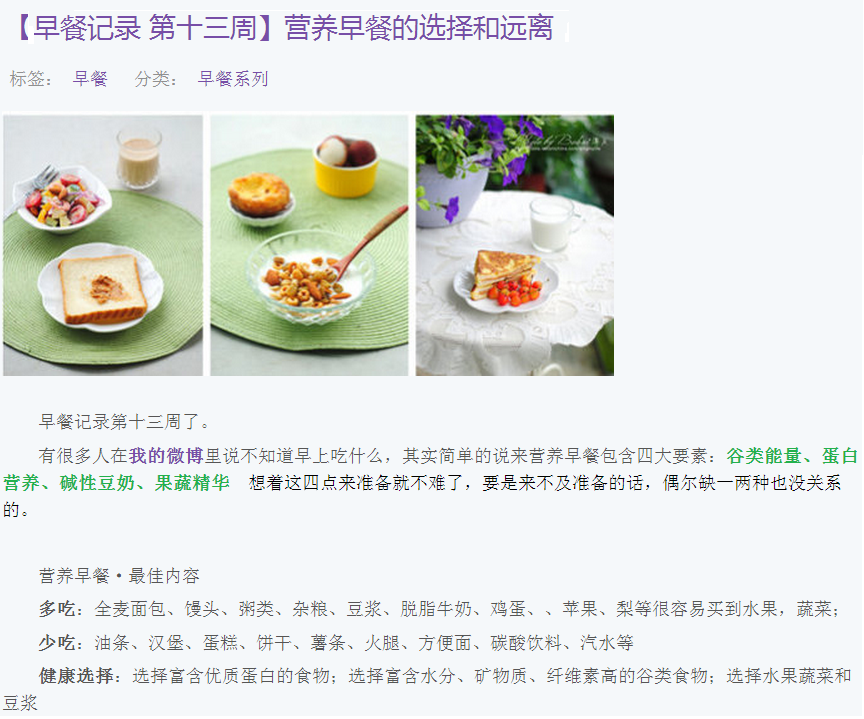
\includegraphics[scale=0.24]{images/breakfast}
\end{center}
\item Information content of any modality is unlikely to be independent of the others.
\item How to dig out the joint representation of multimodal data?
\item How to handle missing data modalities?
\end{itemize}
\end{frame}

\section{Challenges}
\begin{frame}[allowframebreaks]\frametitle{Challenges}
\begin{itemize}
\item Different modalities have different representation.
\centering
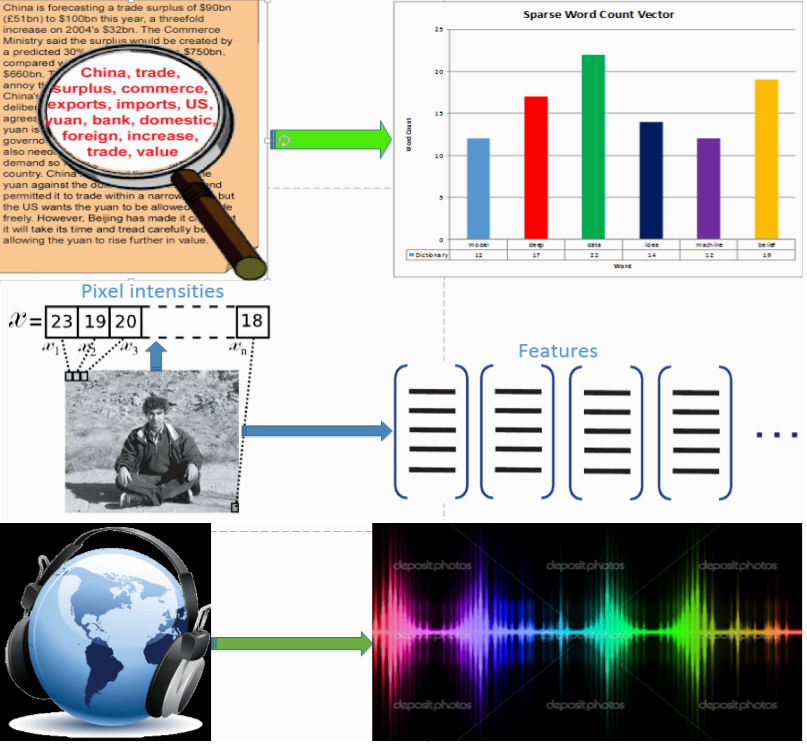
\includegraphics[scale=0.21]{images/multimodaldata}
\item Observations are noisy and may have missing modalities.
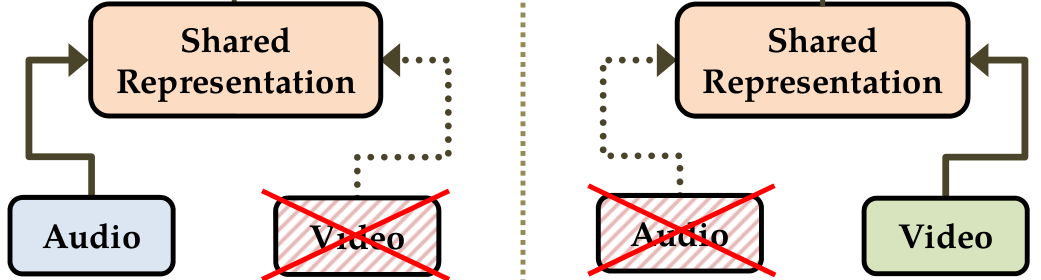
\includegraphics[scale=0.29]{images/missingmodality}
\end{itemize}
\end{frame}


\section{RBMs and relevant Generalizations}
\subsection{Restricted Boltzman Machines}
\begin{frame}
\begin{block}{Restricted Boltzman Machines}
Visible units $v\in\{0,1\}^D$,hidden units $h\in\{0,1\}^F$\\
The \textcolor{blue}{energy} of joint distribution:
\begin{equation}
E(v,h;\theta)=-v^TWh-a^Tv-b^Th
\end{equation}
where $\theta={W,a,b}$ are the model parameters.\\
The \textcolor{blue}{joint probability} over visible and a hidden units:
\begin{equation}
P(v,h;\theta)=\frac{1}{Z(\theta)}\exp(-E(v,h;\theta))
\end{equation}
where $Z(\theta)$ is the normalizing constant:
\begin{equation}
Z(\theta)=\sum_{v,h}\exp(-E(v,h;\theta))
\end{equation}
\end{block}
\end{frame}

\subsection{Multimodal RBM}
\begin{frame}
\begin{block}{Multinomial RBM}
Visible units $v\in \mathbb{N}^K$,hidden units $h\in\{0,1\}^F$.\\
The energy function is defined as follows:
\begin{equation}
E(v,h;\theta)=-\sum_{k=1}^K\sum_{j=1}^Fv_iW_{kj}h_j-\sum_{k=1}^Ka_kv_k-M\sum_{j=1}^Fb_jh_j
\end{equation}
where $v_k$ is frequency of word $k$ in a document,$K$ is vocabulary size,$M=\sum_{k=1}^Kv_k$ is total number of words in the document.\\
This leads to the following conditional distribution:
\begin{equation}
P(v_k=1|h;\theta)=\frac{\exp(-a_k+\sum_{j=1}^FW_{kj}h_j)}{\sum_{k=1}^K\exp(-a_k+\sum_{j=1}^FW_{kj}h_j)}
\end{equation}
\textcolor{red}{Modelling sparse count data,such as word count vectors in a document.}
\end{block}
\end{frame}

\subsection{Gaussian RBM}
\begin{frame}
\begin{block}{Gaussian RBM}
Visible units $v\in \mathbb{R}^D$,hidden units $h\in\{0,1\}^F$.\\
The energy function is defined as follows:
\begin{equation}
E(v,h;\theta)=\sum_{i=1}^D\frac{(v_i-a_i)^2}{2\sigma_i^2}-\sum_{j=1}^Fb_jh_j-\sum_{i,j}\frac{v_i}{\sigma_i}h_jW_{ij}
\end{equation}
where $\theta=\{a,b,W,\sigma\}$ are the model parameters.
This leads to the following conditional distribution:
\begin{equation}
P(v_i,h;\theta)=\mathcal{N}(a_i+\sigma_i\sum_{j=1}^FW_{ij}h_j,\sigma_i^2)
\end{equation}
\textcolor{red}{Modelling real-valued data,such as density value in a image.}
\end{block}
\end{frame}

\section{Multimodal Deep Belief Network}
\subsection{Modality-free Features}
\begin{frame}[allowframebreaks]\frametitle{Modality-free Features}
\textcolor{blue}{Model each data modality using a separate two-layer DBN}.\\
\begin{columns}
\begin{column}{0.5\textwidth}
\centering
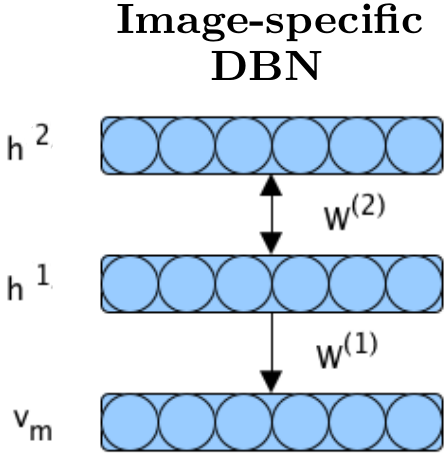
\includegraphics[scale=0.25]{images/imageDBN}
\end{column}
\begin{column}{0.5\textwidth}
\centering
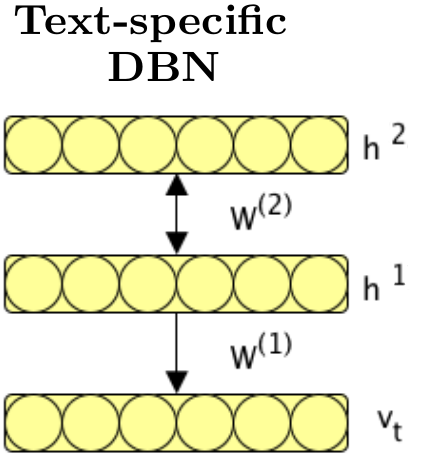
\includegraphics[scale=0.25]{images/textDBN}
\end{column}
\end{columns}

\newpage
Image visible units $v_m\in \mathbb{R}^D$,test visible units $v_t\in \mathbb{N}^K$.\\
\textcolor{blue}{Image-specific DBN} uses Gaussian RBM to model the distribution over real-valued image features:
\begin{equation}
P(v_m)=\sum_{h^1,h^2}P(h^1,h^2)P(v_m|h^1)
\end{equation}
\textcolor{blue}{Text-specific DBN} uses multinomial RBM to model the distribution over word count vectors:
\begin{equation}
P(v_t)=\sum_{h^1,h^2}P(h^1,h^2)P(v_t|h^1)
\end{equation}
\end{frame}

\newpage
\subsection{Multimodal DBN}
\begin{frame}\frametitle{Multimodal DBN}
\textcolor{blue}{Multimodal DBN}:learning a joint RBM on top of two models.\\
\begin{center}
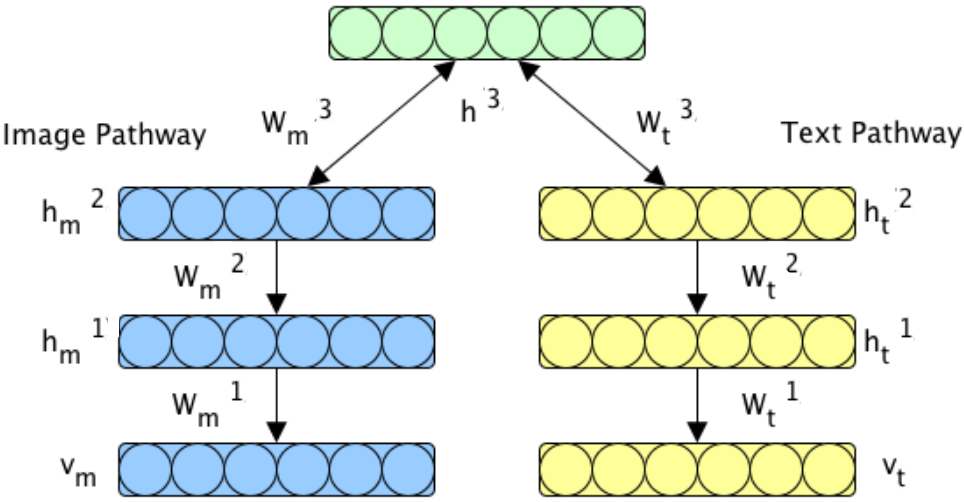
\includegraphics[scale=0.14]{images/multimodal}
\end{center}
The joint distribution can be written as:
\begin{equation}
\begin{split}
P(v_m,v_t)=&\sum_{h_m^2,h_t^2,h^3}P(h_m^2,h_t^2,h^3)\\
&\times \sum_{h_m^1}P(v_m|h_m^1)P(h_m^1|h_m^2)\\
&\times \sum_{h_t^1}P(v_t|h_t^1)P(h_t^1|h_t^2)
\end{split}
\end{equation}
\end{frame}

\subsection{Handle missing modalities}
\begin{frame}[allowframebreaks]\frametitle{Handle missing modalities}
\textcolor{blue}{Infer missing values by drawing samples from conditional model.}\\
\begin{block}{Generate text conditioned on a given image $v_m$}
\begin{enumerate}
\item Infer the values of hidden variables $h_m^2$.
\item Perform Gibbs sampling using following conditional distributions:
\begin{equation}
P(h^3|h_m^2,h_t^2)=\sigma(W_m^3h_m^2+W_t^3h_t^2+b)
\end{equation}
\begin{equation}
P(h_t^2|h^3)=\sigma((W_t^3)^Th^3+a)
\end{equation}
where $\sigma(x)=1/(1+\exp(-x))$.
\item $h_t^2$ can be propagated back to generate text.
\end{enumerate}
\end{block}
\centering
\begin{figure}
\caption[t]{Procedure of infering missing values}
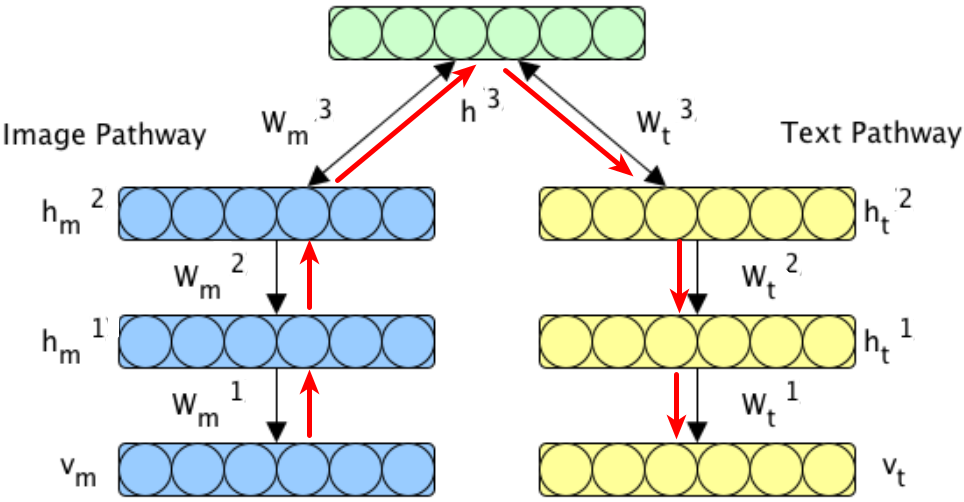
\includegraphics[scale=0.3]{images/infermissingmodality}
\end{figure}

\end{frame}


%\begin{frame}\frametitle{Pseudo-code of the algorithm}
%\begin{algorithm}[H]
%\KwIn{$A \in \mathbb R^{n \times d},Y \in \mathbb R^{d \times N},\rho$;}
%\KwOut{ID(Y);}
%\emph{Set $B=\left[ A^T,\rho I \right],t=0$}\;
%\emph{Initialize $D_t \in \mathbb R^{(n+d) \times (n+d)}$ as an identity matrix}\;
%\Repeat(\tcp*[h]{Iteratively compute U}){Convergence}
%{
%	Calculate $U_{t+1}=D_t^{-1}B^T(BD_t^{-1}B^T)^{-1}Y$\;
%	Calculate the diagonal matrix $D_{t+1}$,where the i-th diagonal element is $\frac{1}{2\|u_{t+1}^t\|_2}$\;
%	$t=t+1$\;
%}
%\For{$j= 1$ \KwTo $N$}
%{
%	Get $r_s(y_j)=\|y-A^T\delta_s(x_j)\|_2,s=1,2,\cdots ,C$\;
%	$ID(y_i)=\mathop{\min}\limits_{s=1,2,\cdots ,C}r_s(y_j)$\;
%}
%\Return $ID(Y)=((ID(y_1),ID(y_2),\cdots ,ID(y_n))$\;	
%\caption{Classification using $\ell_{2,1}$-norm based regression model}
%\end{algorithm}
%\end{frame}
\end{CJK*}
\end{document}
